\subsection{A priori error estimates}

The need for \textit{h-adaptivity} arises from the inefficiency encountered solving the Poisson problem over sequences of uniform meshes while working with pathological exact solutions such as \eqref{pathological_square} and \eqref{pathological_lshape}.

The first step to implement \textit{h-adaptivity} is to evaluate the $\LT$ error on each element and then refine the element with the highest error according to a specific refinement strategy.

The strategy of choice can be outlined as follows:

\begin{enumerate}
    \item For polygons with $N_e \leq 4$, the refiner adds a single node at the polygon's centroid and then connects each edge's midpoint to this new node, creating $N_e$ new quadrilaterals.
    \item For polygons with $N_e > 4$, the refiner adds $N_e$ new nodes at the midpoints of the segments connecting the polygon's centroid to the midpoints of its edges. The refiner then connects these points to form quadrilaterals along the polygon's edges and creates a new smaller polygon by connecting all the new internal nodes.
\end{enumerate}

Refinement occurs by setting a refinement percentage and marking all elements where the local error exceeds that percentage of the highest error. Let $\sigma$ be this percentage, the elements $K$ to be refined are those such that:

\begin{gather}
	\eta_K > \sigma \eta_{M},
\end{gather}

where $\eta_K$ is the local error and $\eta_M$ is the highest error.

Error trends and refined meshes in the following pages. For all the following examples, $\sigma$ is set to $75\%$.

\newpage
\subsubsection{Errors}

The following plots demonstrate that the adaptive approach (red) significantly outperforms uniform refinement (black) when handling these pathological solutions\footnote{$N \in \{125, 250, \dots, 8000\}$ for the uniform meshes.}.

\begin{figure}[!ht]
	\begin{subfigure}[b]{0.45\textwidth}
		% Errors v DOFs template for TikZ.

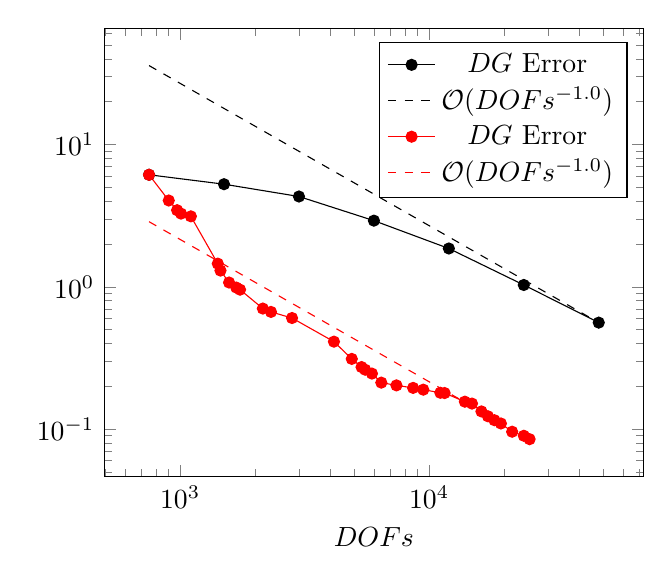
\begin{tikzpicture}
\begin{loglogaxis}[
    xlabel={$DOFs$},
    legend pos=north east,
]

\addplot[black, mark=*] coordinates {(750,6.12566) (1500,5.25995) (3000,4.30988) (6000,2.91652) (12000,1.85839) (24000,1.02974) (48000,0.5601)};
\addlegendentry{$DG$ Error}

\addplot[black, dashed] coordinates {(750,35.8464) (48000,0.5601)};
\addlegendentry{$\mathcal{O}(DOFs^{-1.0})$}

\addplot[red, mark=*] coordinates {(750,6.12566) (900,4.03955) (972,3.45362) (1008,3.26799) (1104,3.12636) (1416,1.45431) (1452,1.30003) (1572,1.0716) (1680,0.987916) (1740,0.954643) (2148,0.70325) (2316,0.666102) (2814,0.603387) (4146,0.411693) (4890,0.311397) (5352,0.272847) (5532,0.261592) (5892,0.245583) (6426,0.212127) (7392,0.202913) (8622,0.194848) (9474,0.189286) (11094,0.180045) (11538,0.179227) (13914,0.155865) (14862,0.151127) (16218,0.133144) (17226,0.123047) (18294,0.11549) (19422,0.109519) (21546,0.0958461) (24006,0.0897779) (25320,0.0849597)};
\addlegendentry{$DG$ Error}

\addplot[red, dashed] coordinates {(750,2.868239472) (25320,0.0849597)};
\addlegendentry{$\mathcal{O}(DOFs^{-1.0})$}

\end{loglogaxis}
\end{tikzpicture}
	\end{subfigure}
	\hfill
	\begin{subfigure}[b]{0.45\textwidth}
		% Errors v DOFs template for TikZ.

\begin{tikzpicture}
\begin{loglogaxis}[
    xlabel={$DOFs$},
    legend pos=north east,
]

\addplot[solarized-base02, mark=*] coordinates {(1250,5.22824) (2500,3.45593) (5000,2.29411) (10000,1.08811) (20000,0.495229) (40000,0.194102) (80000,0.0764724)};
\addlegendentry{$DG$ Error}

\addplot[solarized-base02, dashed] coordinates {(1250,39.1538688) (80000,0.0764724)};
\addlegendentry{$\mathcal{O}(DOFs^{-1.5})$}

\addplot[\accentcolor, mark=*] coordinates {(1250,5.22824) (1450,3.16847) (1570,2.13764) (1690,1.46207) (1750,1.34315) (1800,1.22937) (2280,0.571535) (2400,0.433165) (2720,0.310514) (2950,0.239953) (3240,0.196515) (3470,0.168581) (4650,0.111757) (4830,0.108861) (5260,0.104274) (7150,0.0648557) (7700,0.0513934) (8810,0.0373304) (9890,0.0273954) (10720,0.0239574) (11180,0.0225082) (12420,0.0196702) (16070,0.0156938) (19010,0.0129343) (19560,0.0124709) (20950,0.0102387) (21970,0.00982763) (26960,0.00884522)};
\addlegendentry{$DG$ Error}

\addplot[\accentcolor, dashed] coordinates {(1250,0.8859790477668384) (26960,0.00884522)};
\addlegendentry{$\mathcal{O}(DOFs^{-1.5})$}

\end{loglogaxis}
\end{tikzpicture}
	\end{subfigure}
    \caption{$DG$ errors vs $DOFs$ comparison between adaptively refined meshes and a sequence of uniform meshes over a square domain. $k = 2$ (left), $k = 3$ (right).}
\end{figure}

\begin{figure}[!ht]
	\begin{subfigure}[b]{0.45\textwidth}
		% Errors v DOFs template for TikZ.

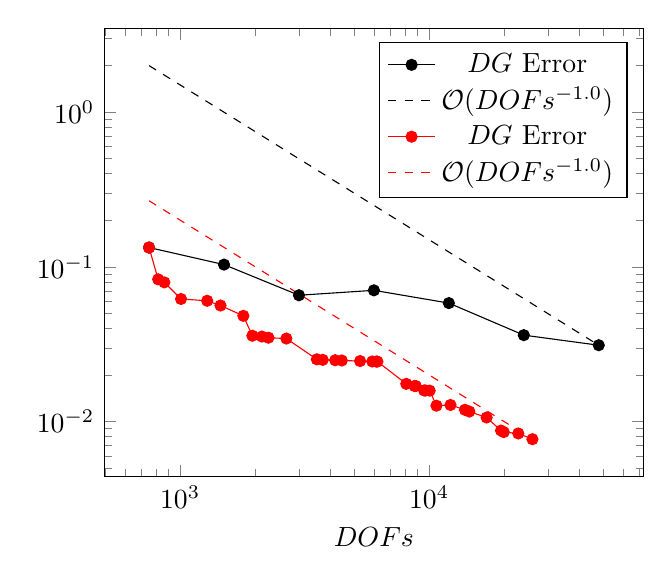
\begin{tikzpicture}
\begin{loglogaxis}[
    xlabel={$DOFs$},
    legend pos=north east,
]

\addplot[black, mark=*] coordinates {(750,0.13327) (1500,0.103364) (3000,0.0655286) (6000,0.0705169) (12000,0.0583046) (24000,0.0362069) (48000,0.0311668)};
\addlegendentry{$DG$ Error}

\addplot[black, dashed] coordinates {(750,1.9946752) (48000,0.0311668)};
\addlegendentry{$\mathcal{O}(DOFs^{-1.0})$}

\addplot[red, mark=*] coordinates {(750,0.13327) (816,0.0830244) (864,0.0793426) (1008,0.0619878) (1284,0.0603523) (1452,0.0562495) (1794,0.0482533) (1950,0.0358904) (2130,0.0354704) (2262,0.0348557) (2670,0.0344147) (3540,0.0252647) (3738,0.0250711) (4194,0.0249254) (4458,0.0248335) (5280,0.0246302) (5910,0.0244758) (6132,0.0244387) (6198,0.0244288) (8094,0.0175423) (8742,0.0169922) (8838,0.0169865) (9546,0.015904) (9660,0.015896) (10050,0.015861) (10698,0.0126811) (12180,0.0128159) (13926,0.0119234) (14502,0.0116229) (17016,0.0106359) (19446,0.00875964) (19938,0.00856267) (22806,0.00838982) (26004,0.00770473)};
\addlegendentry{$DG$ Error}

\addplot[red, dashed] coordinates {(750,0.26713839856000005) (26004,0.00770473)};
\addlegendentry{$\mathcal{O}(DOFs^{-1.0})$}

\end{loglogaxis}
\end{tikzpicture}
	\end{subfigure}
	\hfill
	\begin{subfigure}[b]{0.45\textwidth}
		% Errors v DOFs template for TikZ.

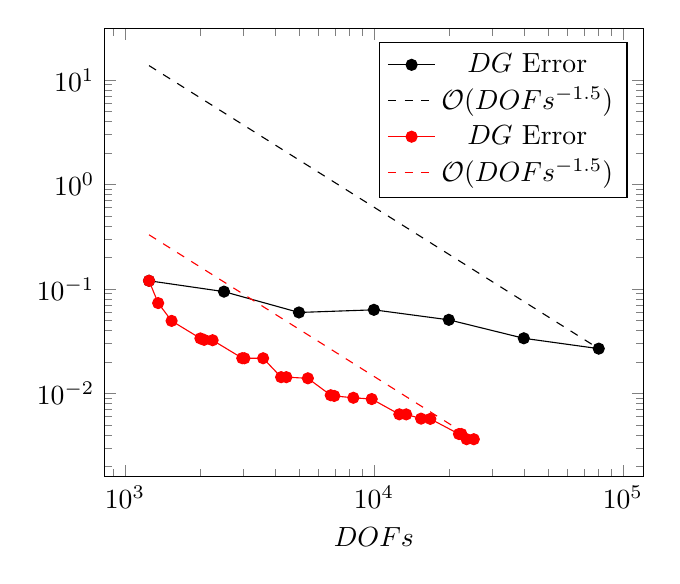
\begin{tikzpicture}
\begin{loglogaxis}[
    xlabel={$DOFs$},
    legend pos=north east,
]

\addplot[black, mark=*] coordinates {(1250,0.119546) (2500,0.0940843) (5000,0.0594572) (10000,0.0630071) (20000,0.050544) (40000,0.0336455) (80000,0.0267768)};
\addlegendentry{$DG$ Error}

\addplot[black, dashed] coordinates {(1250,13.7097216) (80000,0.0267768)};
\addlegendentry{$\mathcal{O}(DOFs^{-1.5})$}

\addplot[red, mark=*] coordinates {(1250,0.119546) (1360,0.0730976) (1540,0.0493759) (2010,0.0335623) (2080,0.0325106) (2250,0.0322421) (2960,0.0217044) (3020,0.0216543) (3590,0.0216774) (4240,0.0142896) (4450,0.0142875) (5430,0.0139307) (6710,0.009591) (6930,0.0094454) (8270,0.00907011) (9800,0.00881814) (12650,0.00629972) (13480,0.00629107) (15470,0.00572756) (16850,0.00569782) (21960,0.00407968) (22460,0.00407912) (23570,0.00364227) (25190,0.00363907)};
\addlegendentry{$DG$ Error}

\addplot[red, dashed] coordinates {(1250,0.3292059237674489) (25190,0.00363907)};
\addlegendentry{$\mathcal{O}(DOFs^{-1.5})$}

\end{loglogaxis}
\end{tikzpicture}
	\end{subfigure}
    \caption{$DG$ errors vs $DOFs$ comparison between adaptively refined meshes and a sequence of uniform meshes over an L-shaped domain. $k = 2$ (left), $k = 3$ (right).}
\end{figure}

\newpage

Due to the nature of the pathological solutions, it may be worth considering adaptive refinement based on local $\HO$ errors rather than $\LT$ errors. The following plots show improved results, particularly for the L-shaped domain.

\begin{figure}[!ht]
	\begin{subfigure}[b]{0.45\textwidth}
		% Errors v DOFs template for TikZ.

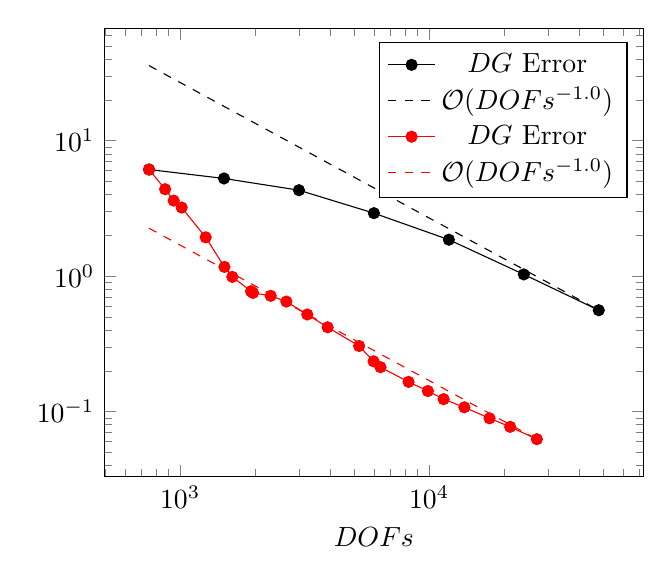
\begin{tikzpicture}
\begin{loglogaxis}[
    xlabel={$DOFs$},
    legend pos=north east,
]

\addplot[black, mark=*] coordinates {(750,6.12566) (1500,5.25995) (3000,4.30988) (6000,2.91652) (12000,1.85839) (24000,1.02974) (48000,0.5601)};
\addlegendentry{$DG$ Error}

\addplot[black, dashed] coordinates {(750,35.8464) (48000,0.5601)};
\addlegendentry{$\mathcal{O}(DOFs^{-1.0})$}

\addplot[red, mark=*] coordinates {(750,6.12566) (870,4.38193) (942,3.60957) (1014,3.20899) (1266,1.93506) (1506,1.16987) (1620,0.987314) (1926,0.773812) (1962,0.752143) (2310,0.715501) (2670,0.648814) (3240,0.520831) (3912,0.419024) (5232,0.304942) (5982,0.234997) (6378,0.212735) (8268,0.165754) (9882,0.141861) (11436,0.123541) (13848,0.107573) (17484,0.0891911) (21156,0.0771805) (27078,0.0625627)};
\addlegendentry{$DG$ Error}

\addplot[red, dashed] coordinates {(750,2.2587637207999998) (27078,0.0625627)};
\addlegendentry{$\mathcal{O}(DOFs^{-1.0})$}

\end{loglogaxis}
\end{tikzpicture}
	\end{subfigure}
	\hfill
	\begin{subfigure}[b]{0.45\textwidth}
		% Errors v DOFs template for TikZ.

\begin{tikzpicture}
\begin{loglogaxis}[
    xlabel={$DOFs$},
    legend pos=north east,
]

\addplot[solarized-base02, mark=*] coordinates {(1250,5.22824) (2500,3.45593) (5000,2.29411) (10000,1.08811) (20000,0.495229) (40000,0.194102) (80000,0.0764724)};
\addlegendentry{$DG$ Error}

\addplot[solarized-base02, dashed] coordinates {(1250,39.1538688) (80000,0.0764724)};
\addlegendentry{$\mathcal{O}(DOFs^{-1.5})$}

\addplot[\accentcolor, mark=*] coordinates {(1250,5.22824) (1450,3.16847) (1570,2.13764) (1690,1.46207) (1800,1.22937) (2220,0.648223) (2340,0.495982) (2600,0.323852) (2770,0.260152) (2880,0.236183) (2950,0.22874) (3530,0.166199) (3760,0.140521) (4530,0.119187) (6130,0.089056) (7600,0.0575574) (8620,0.0390489) (9400,0.0294453) (10160,0.0263927) (10900,0.0229053) (11450,0.0219544) (14750,0.0164373) (17150,0.0131901) (19990,0.0109056) (24140,0.00823295) (27720,0.00688026)};
\addlegendentry{$DG$ Error}

\addplot[\accentcolor, dashed] coordinates {(1250,0.7185047930727512) (27720,0.00688026)};
\addlegendentry{$\mathcal{O}(DOFs^{-1.5})$}

\end{loglogaxis}
\end{tikzpicture}
	\end{subfigure}
    \caption{$DG$ errors vs $DOFs$ comparison between adaptively refined meshes and a sequence of uniform meshes over a square domain. $k = 2$ (left), $k = 3$ (right).}
\end{figure}

\begin{figure}[!ht]
	\begin{subfigure}[b]{0.45\textwidth}
		% Errors v DOFs template for TikZ.

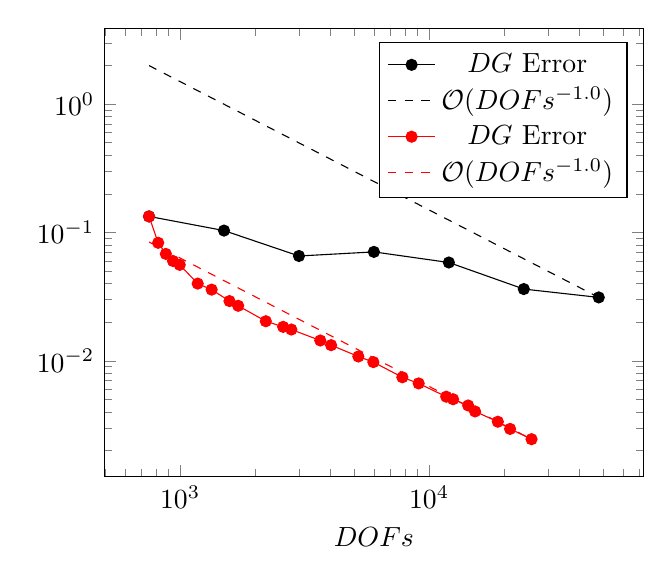
\begin{tikzpicture}
\begin{loglogaxis}[
    xlabel={$DOFs$},
    legend pos=north east,
]

\addplot[black, mark=*] coordinates {(750,0.13327) (1500,0.103364) (3000,0.0655286) (6000,0.0705169) (12000,0.0583046) (24000,0.0362069) (48000,0.0311668)};
\addlegendentry{$DG$ Error}

\addplot[black, dashed] coordinates {(750,1.9946752) (48000,0.0311668)};
\addlegendentry{$\mathcal{O}(DOFs^{-1.0})$}

\addplot[red, mark=*] coordinates {(750,0.13327) (816,0.0830244) (876,0.0680097) (936,0.0598727) (996,0.0559014) (1176,0.039932) (1338,0.0358411) (1578,0.0291867) (1710,0.0268234) (2208,0.0203268) (2592,0.0183746) (2796,0.0175187) (3654,0.0143896) (4038,0.0132366) (5196,0.0107976) (5970,0.00976556) (7806,0.00743953) (9078,0.00666211) (11712,0.00525048) (12480,0.00501671) (14346,0.00448473) (15294,0.00402922) (18876,0.00335053) (21138,0.00294547) (25782,0.00244963)};
\addlegendentry{$DG$ Error}

\addplot[red, dashed] coordinates {(750,0.08420848087999999) (25782,0.00244963)};
\addlegendentry{$\mathcal{O}(DOFs^{-1.0})$}

\end{loglogaxis}
\end{tikzpicture}
	\end{subfigure}
	\hfill
	\begin{subfigure}[b]{0.45\textwidth}
		% Errors v DOFs template for TikZ.

\begin{tikzpicture}
\begin{loglogaxis}[
    xlabel={$DOFs$},
    legend pos=north east,
]

\addplot[solarized-base02, mark=*] coordinates {(1250,0.119546) (2500,0.0940843) (5000,0.0594572) (10000,0.0630071) (20000,0.050544) (40000,0.0336455) (80000,0.0267768)};
\addlegendentry{$DG$ Error}

\addplot[solarized-base02, dashed] coordinates {(1250,13.7097216) (80000,0.0267768)};
\addlegendentry{$\mathcal{O}(DOFs^{-1.5})$}

\addplot[\accentcolor, mark=*] coordinates {(1250,0.119546) (1360,0.0730976) (1460,0.0508708) (1560,0.0375773) (1660,0.0299764) (1760,0.0257653) (1860,0.0238484) (2080,0.0191889) (2220,0.0147015) (2460,0.0125616) (2880,0.00998454) (3190,0.00786125) (3510,0.00673439) (4350,0.0050375) (5080,0.00411082) (6350,0.00313077) (7220,0.00272903) (8830,0.00208062) (10660,0.0015255) (11750,0.00129659) (14290,0.00101426) (16760,0.000817683)};
\addlegendentry{$DG$ Error}

\addplot[\accentcolor, dashed] coordinates {(1250,0.0401449545527477) (16760,0.000817683)};
\addlegendentry{$\mathcal{O}(DOFs^{-1.5})$}

\end{loglogaxis}
\end{tikzpicture} % Incomplete.
	\end{subfigure}
    \caption{$DG$ errors vs $DOFs$ comparison between adaptively refined meshes and a sequence of uniform meshes over an L-shaped domain. $k = 2$ (left), $k = 3$ (right).}
\end{figure}

\newpage
\subsubsection{Meshes}

Due to localized errors, the meshes are refined in areas where the error is greatest, thereby minimizing the number of degrees of freedom in regions where the solution is already well-approximated.

\begin{figure}[!ht]
	\centering
	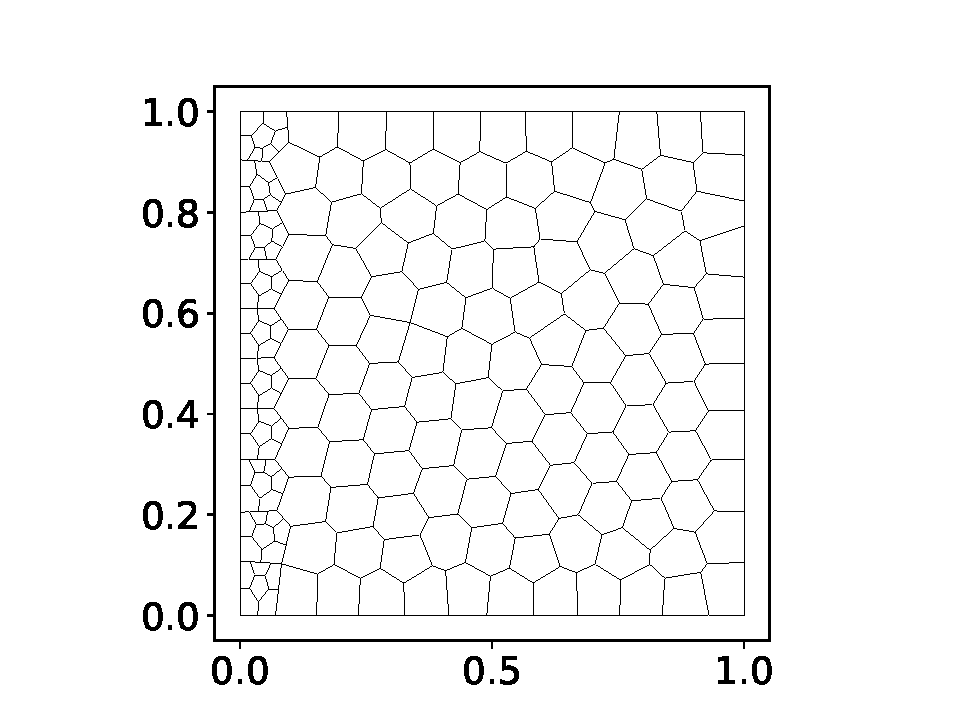
\includegraphics[width=5.5cm]{meshes/adaptive/square_h_5.pdf}
	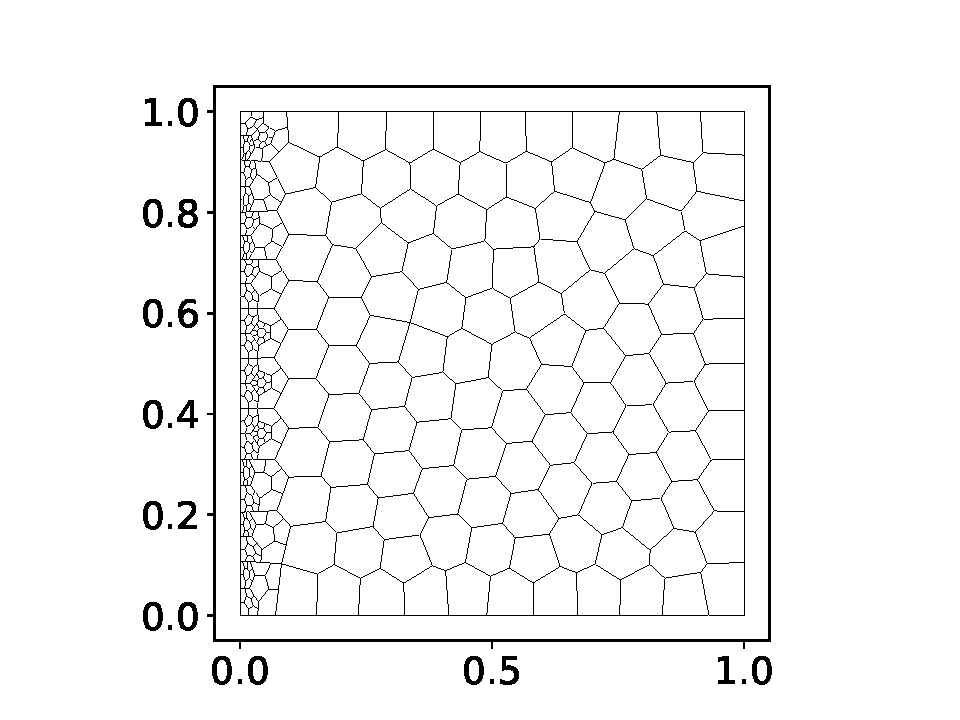
\includegraphics[width=5.5cm]{meshes/adaptive/square_h_10.pdf}
	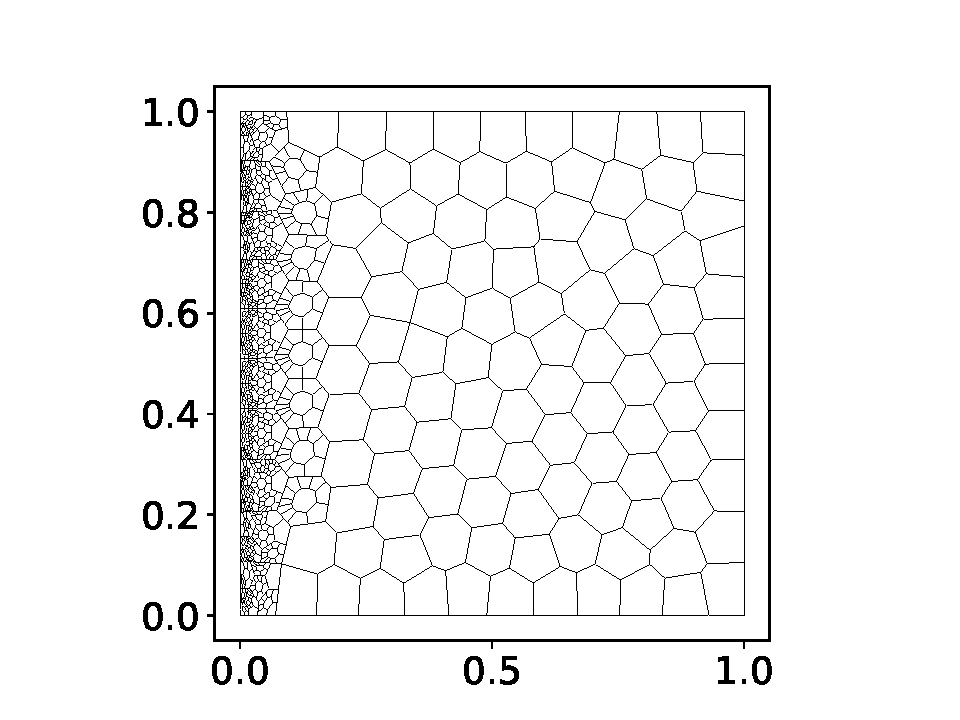
\includegraphics[width=5.5cm]{meshes/adaptive/square_h_20.pdf}
	\caption{Square mesh after 5, 10 and 20 refinements, $N_0 = 125$.}
\end{figure}

\begin{figure}[!ht]
	\centering
	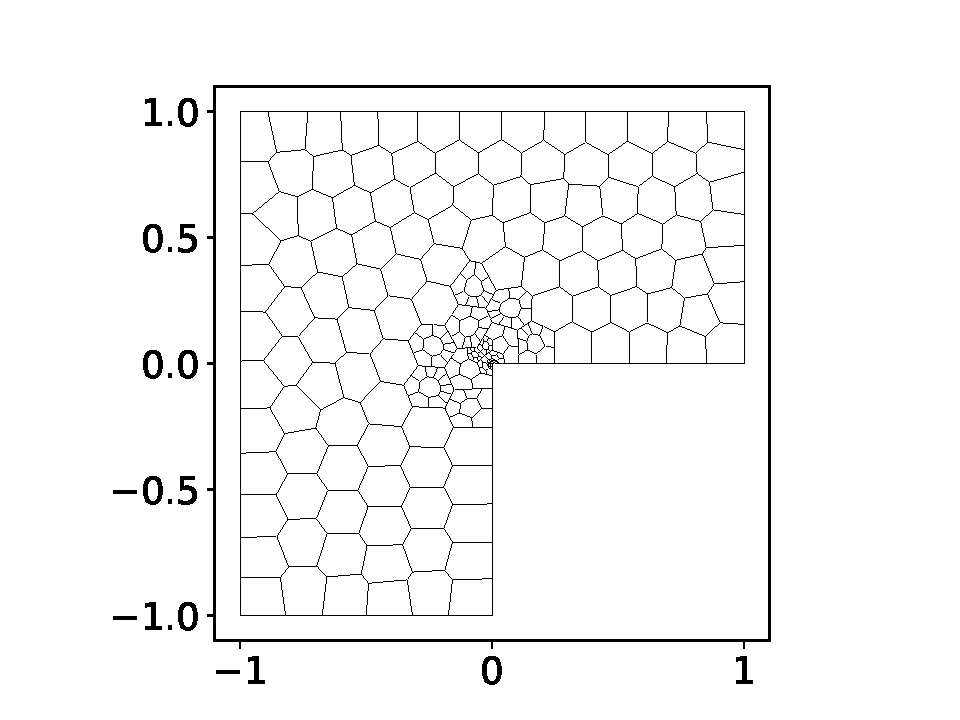
\includegraphics[width=5.5cm]{meshes/adaptive/lshape_h_5.pdf}
	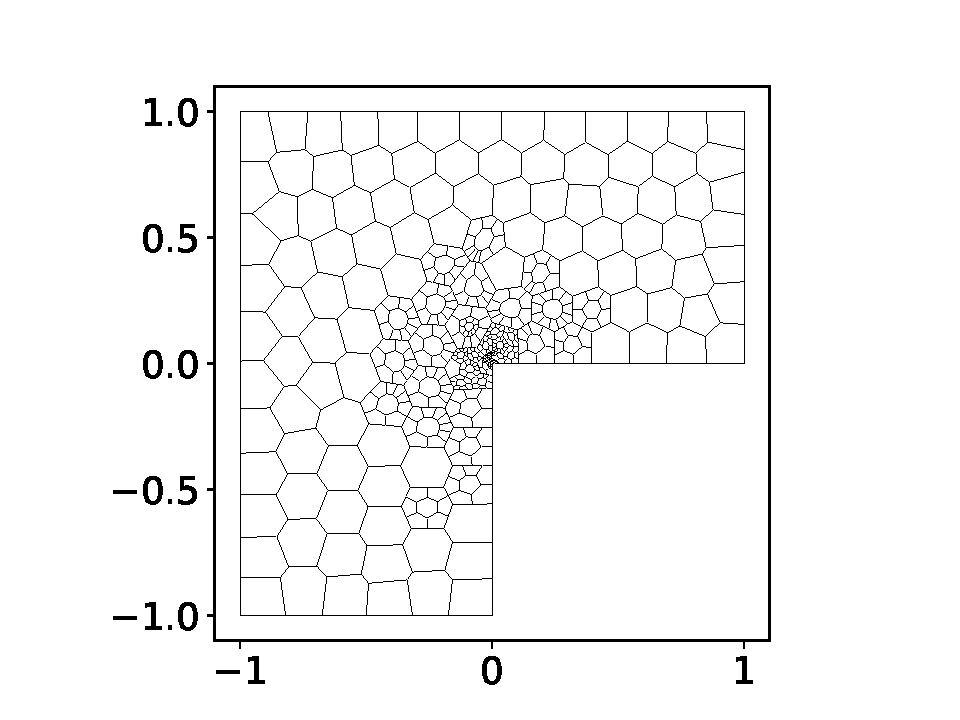
\includegraphics[width=5.5cm]{meshes/adaptive/lshape_h_10.pdf}
	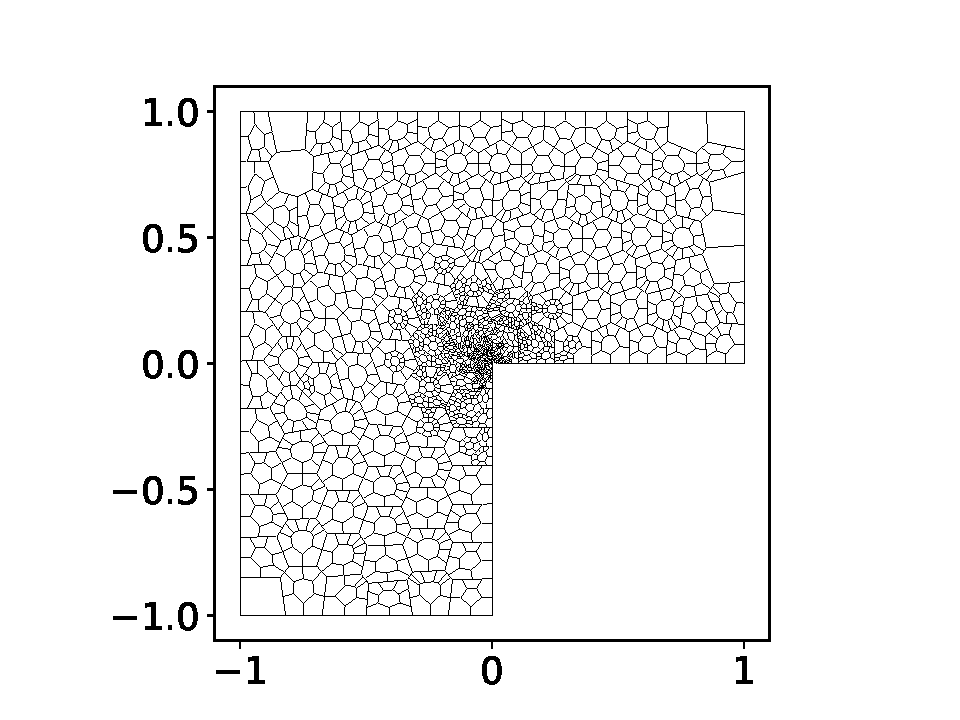
\includegraphics[width=5.5cm]{meshes/adaptive/lshape_h_20.pdf}
	\caption{L-shaped mesh after 5, 10 and 20 refinements, $N_0 = 125$.}
\end{figure}

\newpage

Meshes refined based on local $\HO$ errors exhibit more concentrated refinement, demonstrating once again the superior approach provided by $\HO$ errors for these particular solutions.

\begin{figure}[!ht]
	\centering
	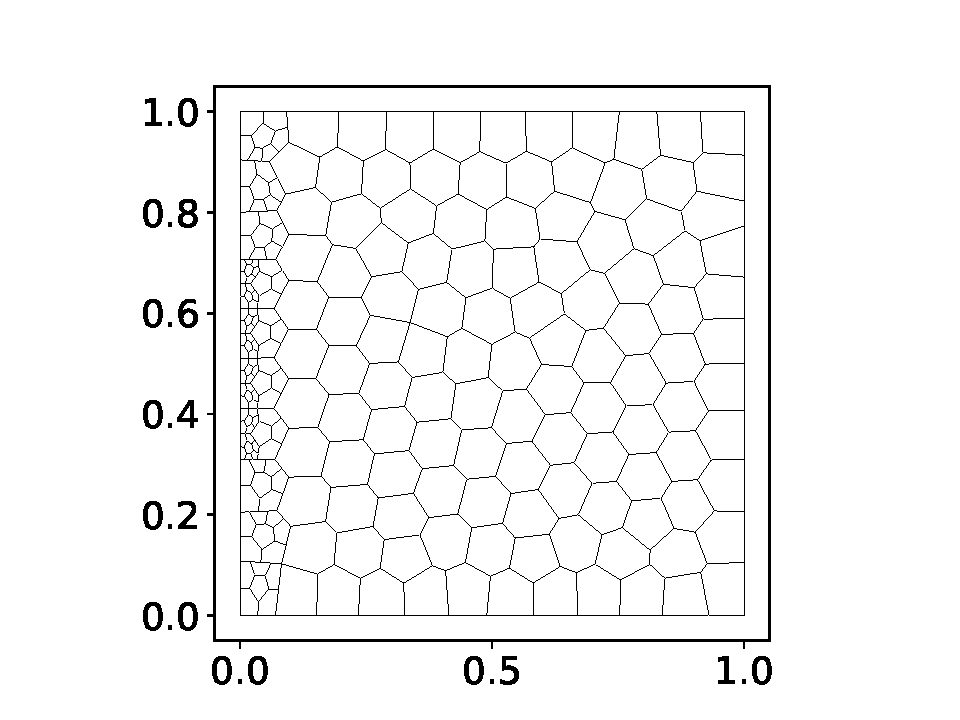
\includegraphics[width=5.5cm]{meshes/adaptive/square_gh_5.pdf}
	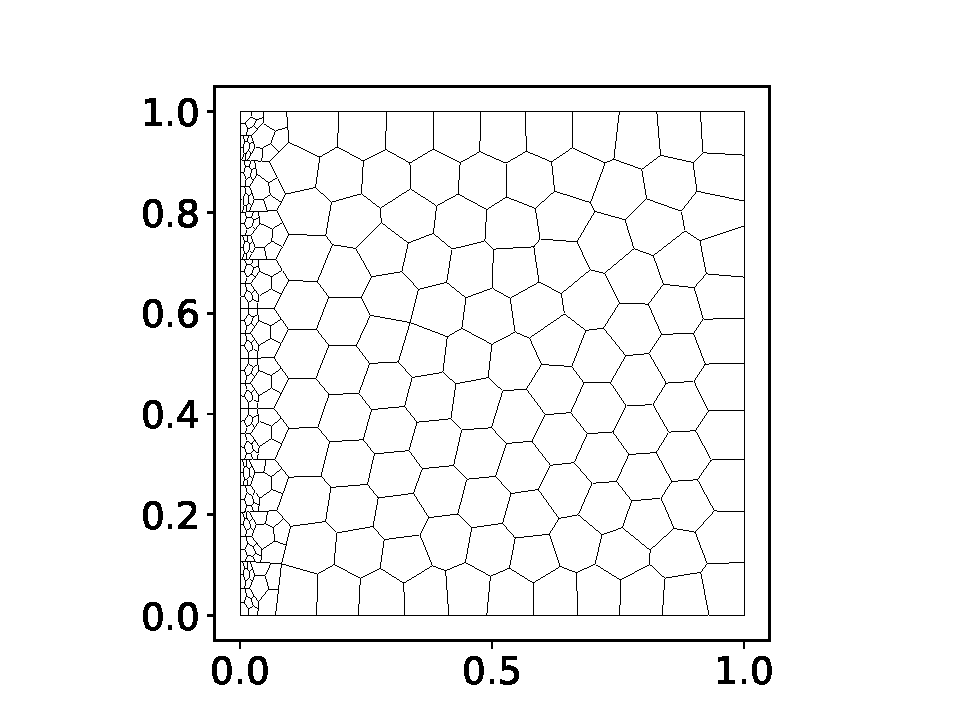
\includegraphics[width=5.5cm]{meshes/adaptive/square_gh_10.pdf}
	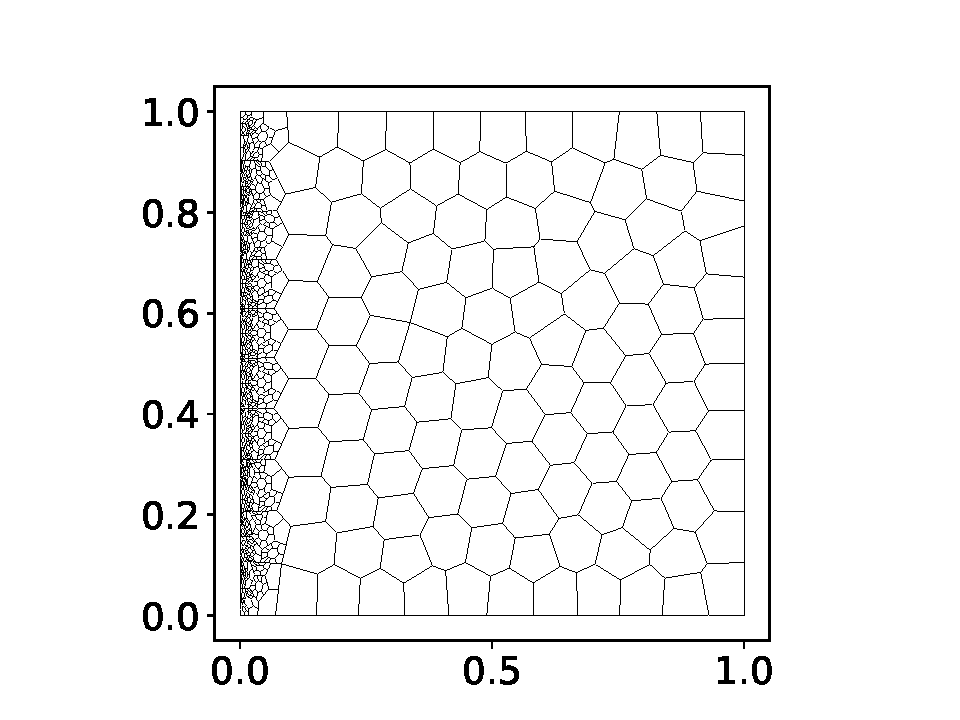
\includegraphics[width=5.5cm]{meshes/adaptive/square_gh_20.pdf}
	\caption{Square mesh after 5, 10 and 20 refinements, $N_0 = 125$.}
\end{figure}

\begin{figure}[!ht]
	\centering
	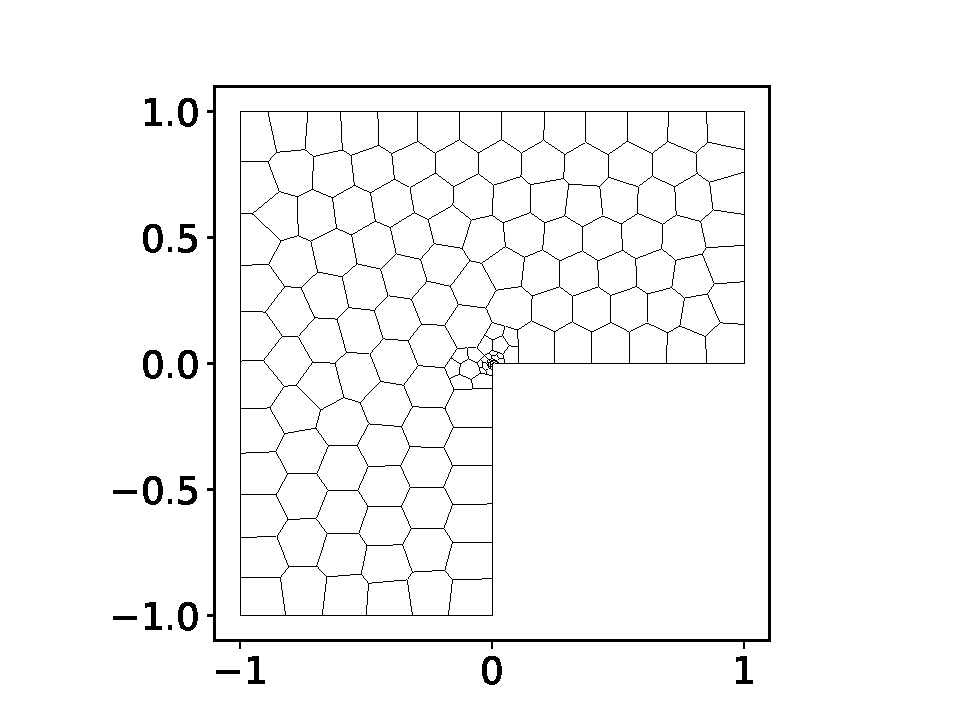
\includegraphics[width=5.5cm]{meshes/adaptive/lshape_gh_5.pdf}
	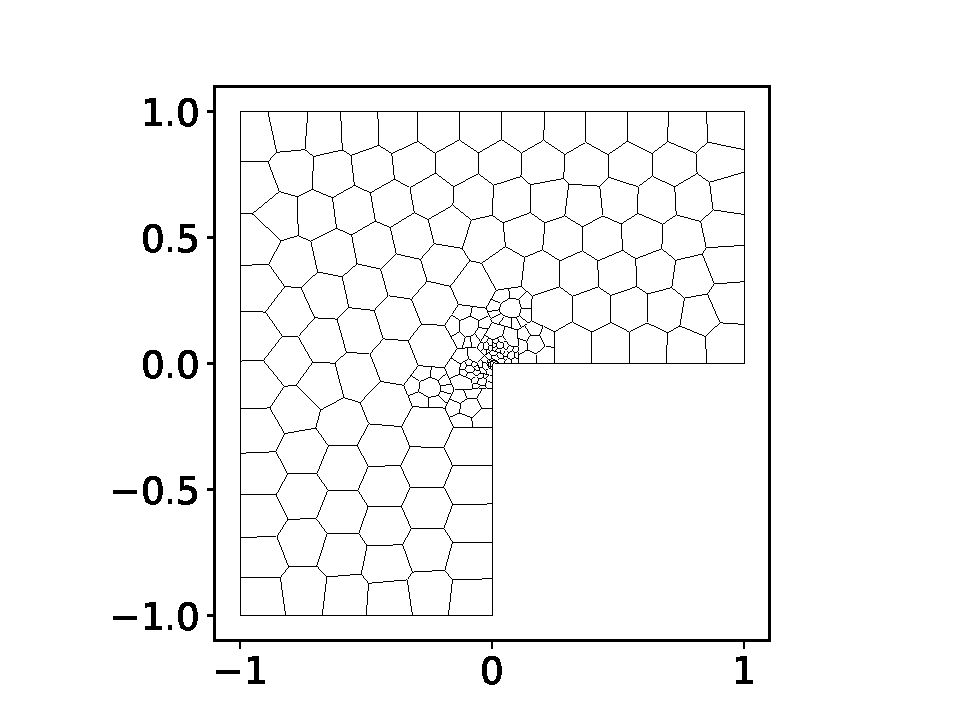
\includegraphics[width=5.5cm]{meshes/adaptive/lshape_gh_10.pdf}
	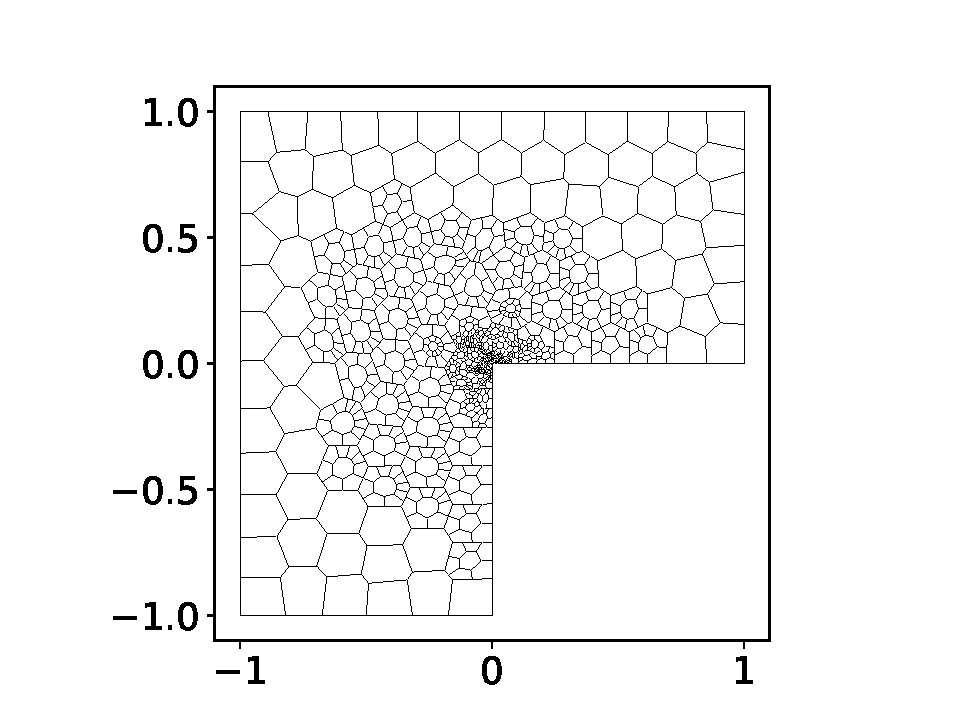
\includegraphics[width=5.5cm]{meshes/adaptive/lshape_gh_20.pdf}
	\caption{L-shaped mesh after 5, 10 and 20 refinements, $N_0 = 125$.}
\end{figure}

\newpage
\subsection{A posteriori error estimates}

The second step to implement \textit{h-adaptivity} is to define an \textit{a posteriori} error estimator, enabling the identification of elements that need refinement without requiring any information about the exact solution.

\cite{Cangiani2023} One possible approach considers the following upper bound on the error:

\begin{gather}
	\lVert u - u^k_h \rVert_{\LT(\Omega)} \leq C_{ub} \sum_{K \in \Tau_h} (R_K^2 + O_K^2),
\end{gather}

where:

\begin{gather}
	R_K^2 = R_{K, E}^2 + R_{K, N}^2 + R_{K, J}^2 + R_{K, T}^2
\end{gather}

is the local estimator and:

\begin{gather}
	O_K^2 = O_{K, E}^2 + O_{K, J}^2 + O_{K, T}^2
\end{gather}

is the local data oscillation, with each term given by:

\begin{align}
	R_{K, E} &= \lVert h (\bar{f} + \Delta u^k_h) \rVert_{\LT(K)}, \\
	R_{K, N} &= \lVert h^{1/2} \llbracket \grad u^k_h \cdot \Vector{n} \rrbracket \rVert_{\LT(\partial K)}, \\
	R^2_{K, J} &= \lVert \sigma^{1/2} \llbracket u^k_h \rrbracket \rVert^2_{\LT(\partial K \cap \Gamma_{i})} + \lVert \sigma^{1/2} (u^k_h - \bar{g}) \rVert^2_{\LT(\partial K \cap \partial \Omega)}, \\
	R^2_{K, T} &= \lVert h^{1/2} \llbracket \grad u^k_h \cdot \Vector{e} \rrbracket \rVert^2_{\LT(\partial K \cap \Gamma_{i})} + \lVert \sigma^{1/2} \grad (u^k_h - \bar{g}) \cdot \Vector{e} \rVert^2_{\LT(\partial K \cap \partial \Omega)}, \\
	O_{K, E} &= \lVert h (f - \bar{f}) \rVert_{\LT(K)}, \\
	O_{K, J} &= \lVert \sigma^{1/2} (g - \bar{g}) \rVert_{\LT(\partial K \cap \partial \Omega)}, \\
	O_{K, T} &= \lVert h^{1/2} \grad (g - \bar{g}) \cdot \Vector{e} \rVert_{\LT(\partial K \cap \partial \Omega)}.
\end{align}

Here, $h$ represents the element size, $\sigma$ denotes the penalty coefficient for a given edge, and $\Vector{e}$ represents the unit vector along a given edge for tangent gradients.

\newpage
\subsubsection{Errors}

These error trends demonstrate that the \textit{a posteriori} error estimates (red) behave similarly to the \textit{a priori} estimates (black). Additionally, in the case of the L-shaped domain, they exhibit improved behavior due to more concentrated refinement in the region of greatest interest. This is due to the significant local data oscillation caused by the singularity of $\grad u$ at the origin for this particular pathological solution.

\begin{figure}[!ht]
	\begin{subfigure}[b]{0.45\textwidth}
		% Errors v DOFs template for TikZ.

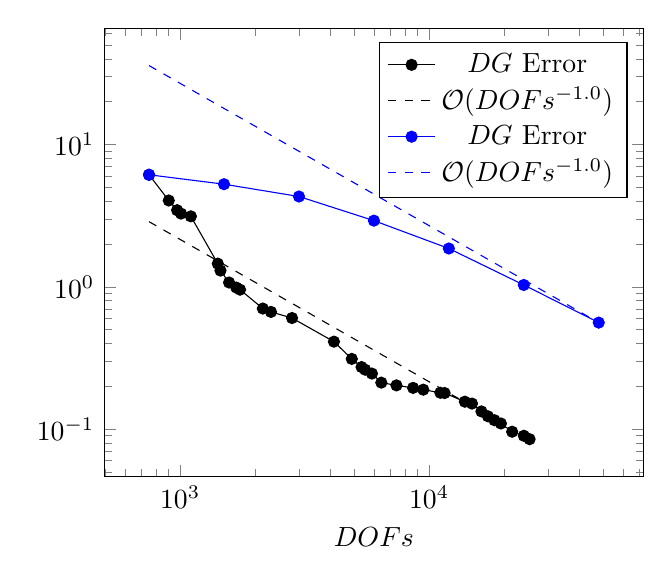
\begin{tikzpicture}
\begin{loglogaxis}[
    xlabel={$DOFs$},
    legend pos=north east,
]

\addplot[black, mark=*] coordinates {(750,6.12566) (900,4.03955) (972,3.45362) (1008,3.26799) (1104,3.12636) (1416,1.45431) (1452,1.30003) (1572,1.0716) (1680,0.987916) (1740,0.954643) (2148,0.70325) (2316,0.666102) (2814,0.603387) (4146,0.411693) (4890,0.311397) (5352,0.272847) (5532,0.261592) (5892,0.245583) (6426,0.212127) (7392,0.202913) (8622,0.194848) (9474,0.189286) (11094,0.180045) (11538,0.179227) (13914,0.155865) (14862,0.151127) (16218,0.133144) (17226,0.123047) (18294,0.11549) (19422,0.109519) (21546,0.0958461) (24006,0.0897779) (25320,0.0849597)};
\addlegendentry{$DG$ Error}

\addplot[black, dashed] coordinates {(750,2.868239472) (25320,0.0849597)};
\addlegendentry{$\mathcal{O}(DOFs^{-1.0})$}

\addplot[blue, mark=*] coordinates {(750,6.12566) (1500,5.25995) (3000,4.30988) (6000,2.91652) (12000,1.85839) (24000,1.02974) (48000,0.5601)};
\addlegendentry{$DG$ Error}

\addplot[blue, dashed] coordinates {(750,35.8464) (48000,0.5601)};
\addlegendentry{$\mathcal{O}(DOFs^{-1.0})$}

\end{loglogaxis}
\end{tikzpicture}
	\end{subfigure}
	\hfill
	\begin{subfigure}[b]{0.45\textwidth}
		% Errors v DOFs template for TikZ.

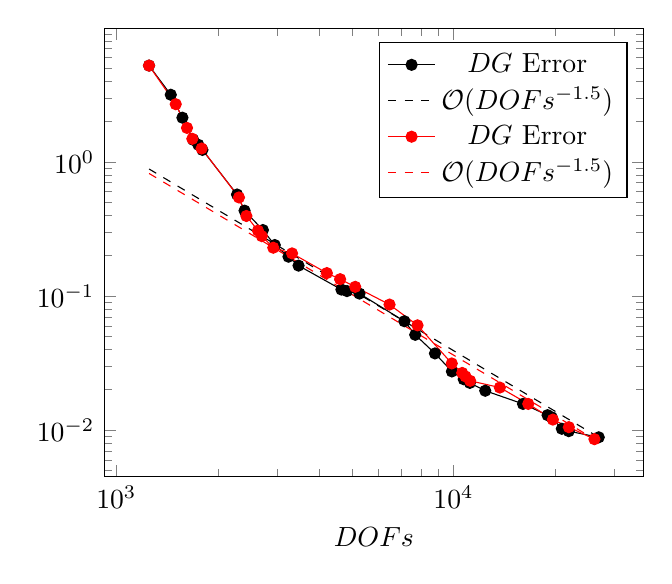
\begin{tikzpicture}
\begin{loglogaxis}[
    xlabel={$DOFs$},
    legend pos=north east,
]

\addplot[black, mark=*] coordinates {(1250,5.22824) (1450,3.16847) (1570,2.13764) (1690,1.46207) (1750,1.34315) (1800,1.22937) (2280,0.571535) (2400,0.433165) (2720,0.310514) (2950,0.239953) (3240,0.196515) (3470,0.168581) (4650,0.111757) (4830,0.108861) (5260,0.104274) (7150,0.0648557) (7700,0.0513934) (8810,0.0373304) (9890,0.0273954) (10720,0.0239574) (11180,0.0225082) (12420,0.0196702) (16070,0.0156938) (19010,0.0129343) (19560,0.0124709) (20950,0.0102387) (21970,0.00982763) (26960,0.00884522)};
\addlegendentry{$DG$ Error}

\addplot[black, dashed] coordinates {(1250,0.8859790477668384) (26960,0.00884522)};
\addlegendentry{$\mathcal{O}(DOFs^{-1.5})$}

\addplot[red, mark=*] coordinates {(1250,5.22824) (1500,2.69514) (1620,1.7934) (1680,1.48702) (1790,1.25894) (2310,0.543447) (2430,0.395368) (2630,0.307434) (2700,0.279644) (2920,0.229209) (3320,0.207952) (4210,0.148303) (4610,0.133591) (5110,0.117099) (6460,0.0863494) (7820,0.0604748) (9880,0.0314321) (10610,0.0267064) (10850,0.0251548) (11200,0.0233236) (13720,0.0207803) (16660,0.0156883) (19710,0.0119851) (21980,0.0105234) (26180,0.00856227)};
\addlegendentry{$DG$ Error}

\addplot[red, dashed] coordinates {(1250,0.8206885275389775) (26180,0.00856227)};
\addlegendentry{$\mathcal{O}(DOFs^{-1.5})$}

\end{loglogaxis}
\end{tikzpicture}
	\end{subfigure}
    \caption{$DG$ errors vs $DOFs$ comparison between adaptively refined meshes over a square domain. $k = 2$ (left), $k = 3$ (right).}
\end{figure}

\begin{figure}[!ht]
	\begin{subfigure}[b]{0.45\textwidth}
		% Errors v DOFs template for TikZ.

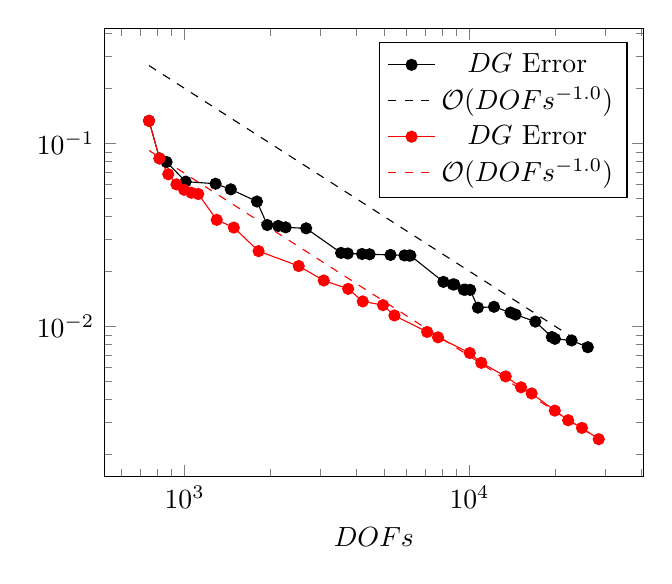
\begin{tikzpicture}
\begin{loglogaxis}[
    xlabel={$DOFs$},
    legend pos=north east,
]

\addplot[black, mark=*] coordinates {(750,0.13327) (816,0.0830244) (864,0.0793426) (1008,0.0619878) (1284,0.0603523) (1452,0.0562495) (1794,0.0482533) (1950,0.0358904) (2130,0.0354704) (2262,0.0348557) (2670,0.0344147) (3540,0.0252647) (3738,0.0250711) (4194,0.0249254) (4458,0.0248335) (5280,0.0246302) (5910,0.0244758) (6132,0.0244387) (6198,0.0244288) (8094,0.0175423) (8742,0.0169922) (8838,0.0169865) (9546,0.015904) (9660,0.015896) (10050,0.015861) (10698,0.0126811) (12180,0.0128159) (13926,0.0119234) (14502,0.0116229) (17016,0.0106359) (19446,0.00875964) (19938,0.00856267) (22806,0.00838982) (26004,0.00770473)};
\addlegendentry{$DG$ Error}

\addplot[black, dashed] coordinates {(750,0.26713839856000005) (26004,0.00770473)};
\addlegendentry{$\mathcal{O}(DOFs^{-1.0})$}

\addplot[red, mark=*] coordinates {(750,0.13327) (816,0.0830244) (876,0.0680097) (936,0.0598727) (996,0.0559014) (1056,0.0538816) (1116,0.0530303) (1296,0.0382955) (1488,0.0347494) (1818,0.0258365) (2514,0.021412) (3078,0.0178477) (3750,0.0160642) (4218,0.0137184) (4968,0.0130898) (5448,0.0114913) (7098,0.0093373) (7752,0.00872489) (10020,0.007165) (10998,0.00633046) (13392,0.00533555) (15168,0.00465232) (16518,0.00430527) (19920,0.00346828) (22188,0.00307256) (24804,0.00278921) (28410,0.00242059)};
\addlegendentry{$DG$ Error}

\addplot[red, dashed] coordinates {(750,0.0916919492) (28410,0.00242059)};
\addlegendentry{$\mathcal{O}(DOFs^{-1.0})$}

\end{loglogaxis}
\end{tikzpicture}
	\end{subfigure}
	\hfill
	\begin{subfigure}[b]{0.45\textwidth}
		% Errors v DOFs template for TikZ.

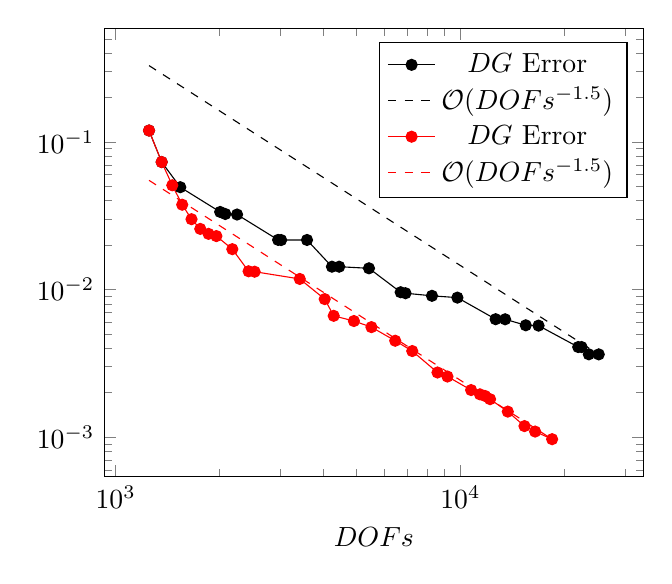
\begin{tikzpicture}
\begin{loglogaxis}[
    xlabel={$DOFs$},
    legend pos=north east,
]

\addplot[black, mark=*] coordinates {(1250,0.119546) (1360,0.0730976) (1540,0.0493759) (2010,0.0335623) (2080,0.0325106) (2250,0.0322421) (2960,0.0217044) (3020,0.0216543) (3590,0.0216774) (4240,0.0142896) (4450,0.0142875) (5430,0.0139307) (6710,0.009591) (6930,0.0094454) (8270,0.00907011) (9800,0.00881814) (12650,0.00629972) (13480,0.00629107) (15470,0.00572756) (16850,0.00569782) (21960,0.00407968) (22460,0.00407912) (23570,0.00364227) (25190,0.00363907)};
\addlegendentry{$DG$ Error}

\addplot[black, dashed] coordinates {(1250,0.3292059237674489) (25190,0.00363907)};
\addlegendentry{$\mathcal{O}(DOFs^{-1.5})$}

\addplot[red, mark=*] coordinates {(1250,0.119546) (1360,0.0730976) (1460,0.0508708) (1560,0.0375773) (1660,0.0299764) (1760,0.0257653) (1860,0.0238484) (1960,0.0230301) (2180,0.0187842) (2430,0.0133021) (2530,0.0132102) (3420,0.0118042) (4040,0.00861783) (4290,0.00663868) (4910,0.00612195) (5520,0.00556495) (6470,0.00450029) (7250,0.00383231) (8580,0.00274332) (9170,0.00257528) (10740,0.00208511) (11390,0.0019513) (11790,0.00190163) (12190,0.0018094) (13720,0.00149002) (15340,0.00118862) (16470,0.00109125) (18450,0.000969034)};
\addlegendentry{$DG$ Error}

\addplot[red, dashed] coordinates {(1250,0.054950108137377836) (18450,0.000969034)};
\addlegendentry{$\mathcal{O}(DOFs^{-1.5})$}

\end{loglogaxis}
\end{tikzpicture} % Incomplete.
	\end{subfigure}
    \caption{$DG$ errors vs $DOFs$ comparison between adaptively refined meshes over an L-shaped domain. $k = 2$ (left), $k = 3$ (right).}
\end{figure}

\newpage

A better comparison can be made with respect to the $\HO$ refinement, for which the \textit{a posteriori} estimates exhibit the same behavior.

\begin{figure}[!ht]
	\begin{subfigure}[b]{0.45\textwidth}
		% Errors v DOFs template for TikZ.

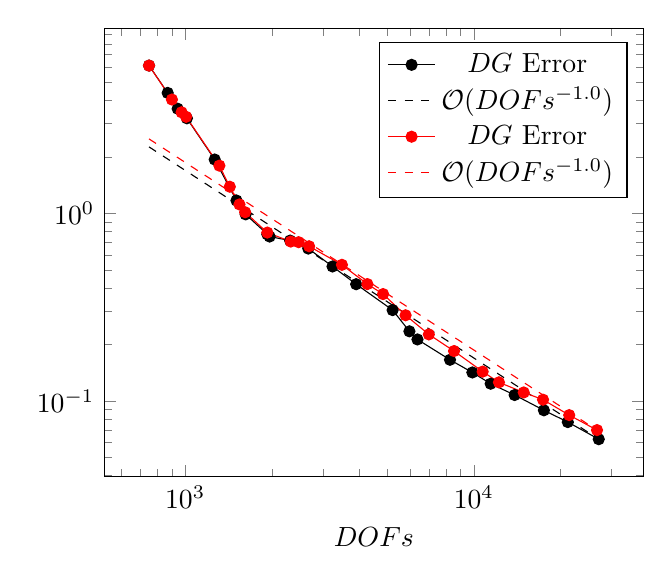
\begin{tikzpicture}
\begin{loglogaxis}[
    xlabel={$DOFs$},
    legend pos=north east,
]

\addplot[black, mark=*] coordinates {(750,6.12566) (870,4.38193) (942,3.60957) (1014,3.20899) (1266,1.93506) (1506,1.16987) (1620,0.987314) (1926,0.773812) (1962,0.752143) (2310,0.715501) (2670,0.648814) (3240,0.520831) (3912,0.419024) (5232,0.304942) (5982,0.234997) (6378,0.212735) (8268,0.165754) (9882,0.141861) (11436,0.123541) (13848,0.107573) (17484,0.0891911) (21156,0.0771805) (27078,0.0625627)};
\addlegendentry{$DG$ Error}

\addplot[black, dashed] coordinates {(750,2.2587637207999998) (27078,0.0625627)};
\addlegendentry{$\mathcal{O}(DOFs^{-1.0})$}

\addplot[red, mark=*] coordinates {(750,6.12566) (900,4.03955) (972,3.45362) (1008,3.26799) (1314,1.79461) (1428,1.38556) (1542,1.11532) (1614,1.01291) (1926,0.78948) (2322,0.707091) (2472,0.701825) (2688,0.667295) (3492,0.531519) (4278,0.419556) (4848,0.371234) (5802,0.286217) (6984,0.22631) (8538,0.184473) (10728,0.143353) (12216,0.125698) (14886,0.111004) (17364,0.101579) (21396,0.0840658) (26706,0.0699521)};
\addlegendentry{$DG$ Error}

\addplot[red, dashed] coordinates {(750,2.4908543767999998) (26706,0.0699521)};
\addlegendentry{$\mathcal{O}(DOFs^{-1.0})$}

\end{loglogaxis}
\end{tikzpicture}
	\end{subfigure}
	\hfill
	\begin{subfigure}[b]{0.45\textwidth}
		% Errors v DOFs template for TikZ.

\begin{tikzpicture}
\begin{loglogaxis}[
    xlabel={$DOFs$},
    legend pos=north east,
]

\addplot[solarized-base02, mark=*] coordinates {(1250,5.22824) (1450,3.16847) (1570,2.13764) (1690,1.46207) (1800,1.22937) (2220,0.648223) (2340,0.495982) (2600,0.323852) (2770,0.260152) (2880,0.236183) (2950,0.22874) (3530,0.166199) (3760,0.140521) (4530,0.119187) (6130,0.089056) (7600,0.0575574) (8620,0.0390489) (9400,0.0294453) (10160,0.0263927) (10900,0.0229053) (11450,0.0219544) (14750,0.0164373) (17150,0.0131901) (19990,0.0109056) (24140,0.00823295) (27720,0.00688026)};
\addlegendentry{$DG$ Error}

\addplot[solarized-base02, dashed] coordinates {(1250,0.7185047930727512) (27720,0.00688026)};
\addlegendentry{$\mathcal{O}(DOFs^{-1.5})$}

\addplot[\accentcolor, mark=*] coordinates {(1250,5.22824) (1500,2.69514) (1620,1.7934) (1680,1.48702) (1790,1.25894) (2310,0.543447) (2430,0.395368) (2630,0.307434) (2700,0.279644) (2920,0.229209) (3320,0.207952) (4210,0.148303) (4610,0.133591) (5110,0.117099) (6460,0.0863494) (7820,0.0604748) (9880,0.0314321) (10610,0.0267064) (10850,0.0251548) (11200,0.0233236) (13720,0.0207803) (16660,0.0156883) (19710,0.0119851) (21980,0.0105234) (26180,0.00856227)};
\addlegendentry{$DG$ Error}

\addplot[\accentcolor, dashed] coordinates {(1250,0.8206885275389775) (26180,0.00856227)};
\addlegendentry{$\mathcal{O}(DOFs^{-1.5})$}

\end{loglogaxis}
\end{tikzpicture}
	\end{subfigure}
    \caption{$DG$ errors vs $DOFs$ comparison between adaptively refined meshes over a square domain. $k = 2$ (left), $k = 3$ (right).}
\end{figure}

\begin{figure}[!ht]
	\begin{subfigure}[b]{0.45\textwidth}
		% Errors v DOFs template for TikZ.

\begin{tikzpicture}
\begin{loglogaxis}[
    xlabel={$DOFs$},
    legend pos=north east,
]

\addplot[solarized-base02, mark=*] coordinates {(750,0.13327) (816,0.0830244) (876,0.0680097) (936,0.0598727) (996,0.0559014) (1176,0.039932) (1338,0.0358411) (1578,0.0291867) (1710,0.0268234) (2208,0.0203268) (2592,0.0183746) (2796,0.0175187) (3654,0.0143896) (4038,0.0132366) (5196,0.0107976) (5970,0.00976556) (7806,0.00743953) (9078,0.00666211) (11712,0.00525048) (12480,0.00501671) (14346,0.00448473) (15294,0.00402922) (18876,0.00335053) (21138,0.00294547) (25782,0.00244963)};
\addlegendentry{$DG$ Error}

\addplot[solarized-base02, dashed] coordinates {(750,0.08420848087999999) (25782,0.00244963)};
\addlegendentry{$\mathcal{O}(DOFs^{-1.0})$}

\addplot[\accentcolor, mark=*] coordinates {(750,0.13327) (816,0.0830244) (876,0.0680097) (936,0.0598727) (996,0.0559014) (1056,0.0538816) (1116,0.0530303) (1296,0.0382955) (1488,0.0347494) (1818,0.0258365) (2514,0.021412) (3078,0.0178477) (3750,0.0160642) (4218,0.0137184) (4968,0.0130898) (5448,0.0114913) (7098,0.0093373) (7752,0.00872489) (10020,0.007165) (10998,0.00633046) (13392,0.00533555) (15168,0.00465232) (16518,0.00430527) (19920,0.00346828) (22188,0.00307256) (24804,0.00278921) (28410,0.00242059)};
\addlegendentry{$DG$ Error}

\addplot[\accentcolor, dashed] coordinates {(750,0.0916919492) (28410,0.00242059)};
\addlegendentry{$\mathcal{O}(DOFs^{-1.0})$}

\end{loglogaxis}
\end{tikzpicture}
	\end{subfigure}
	\hfill
	\begin{subfigure}[b]{0.45\textwidth}
		% Errors v DOFs template for TikZ.

\begin{tikzpicture}
\begin{loglogaxis}[
    xlabel={$DOFs$},
    legend pos=north east,
]

\addplot[solarized-base02, mark=*] coordinates {(1250,0.119546) (1360,0.0730976) (1460,0.0508708) (1560,0.0375773) (1660,0.0299764) (1760,0.0257653) (1860,0.0238484) (2080,0.0191889) (2220,0.0147015) (2460,0.0125616) (2880,0.00998454) (3190,0.00786125) (3510,0.00673439) (4350,0.0050375) (5080,0.00411082) (6350,0.00313077) (7220,0.00272903) (8830,0.00208062) (10660,0.0015255) (11750,0.00129659) (14290,0.00101426) (16760,0.000817683)};
\addlegendentry{$DG$ Error}

\addplot[solarized-base02, dashed] coordinates {(1250,0.0401449545527477) (16760,0.000817683)};
\addlegendentry{$\mathcal{O}(DOFs^{-1.5})$}

\addplot[\accentcolor, mark=*] coordinates {(1250,0.119546) (1360,0.0730976) (1460,0.0508708) (1560,0.0375773) (1660,0.0299764) (1760,0.0257653) (1860,0.0238484) (1960,0.0230301) (2180,0.0187842) (2430,0.0133021) (2530,0.0132102) (3420,0.0118042) (4040,0.00861783) (4290,0.00663868) (4910,0.00612195) (5520,0.00556495) (6470,0.00450029) (7250,0.00383231) (8580,0.00274332) (9170,0.00257528) (10740,0.00208511) (11390,0.0019513) (11790,0.00190163) (12190,0.0018094) (13720,0.00149002) (15340,0.00118862) (16470,0.00109125) (18450,0.000969034)};
\addlegendentry{$DG$ Error}

\addplot[\accentcolor, dashed] coordinates {(1250,0.054950108137377836) (18450,0.000969034)};
\addlegendentry{$\mathcal{O}(DOFs^{-1.5})$}

\end{loglogaxis}
\end{tikzpicture} % Incomplete.
	\end{subfigure}
    \caption{$DG$ errors vs $DOFs$ comparison between adaptively refined meshes over an L-shaped domain. $k = 2$ (left), $k = 3$ (right).}
\end{figure}

\newpage
\subsubsection{Meshes}

These meshes exhibit a more concentrated refinement compared to those refined using \textit{a priori} error estimates.

\begin{figure}[!ht]
	\centering
	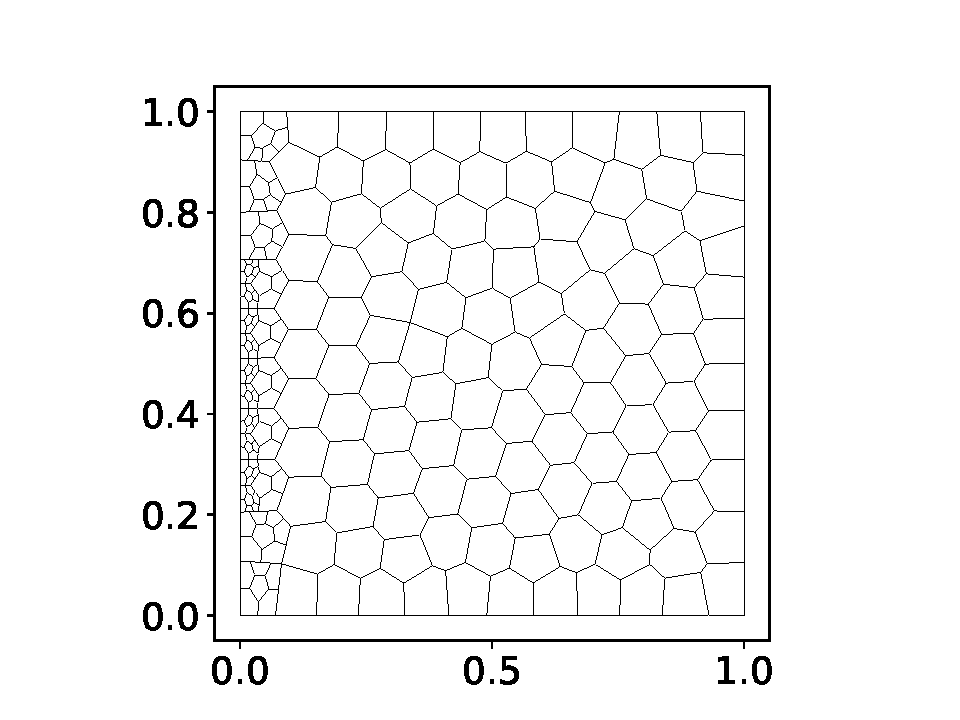
\includegraphics[width=5.5cm]{meshes/adaptive/square_eh_5.pdf}
	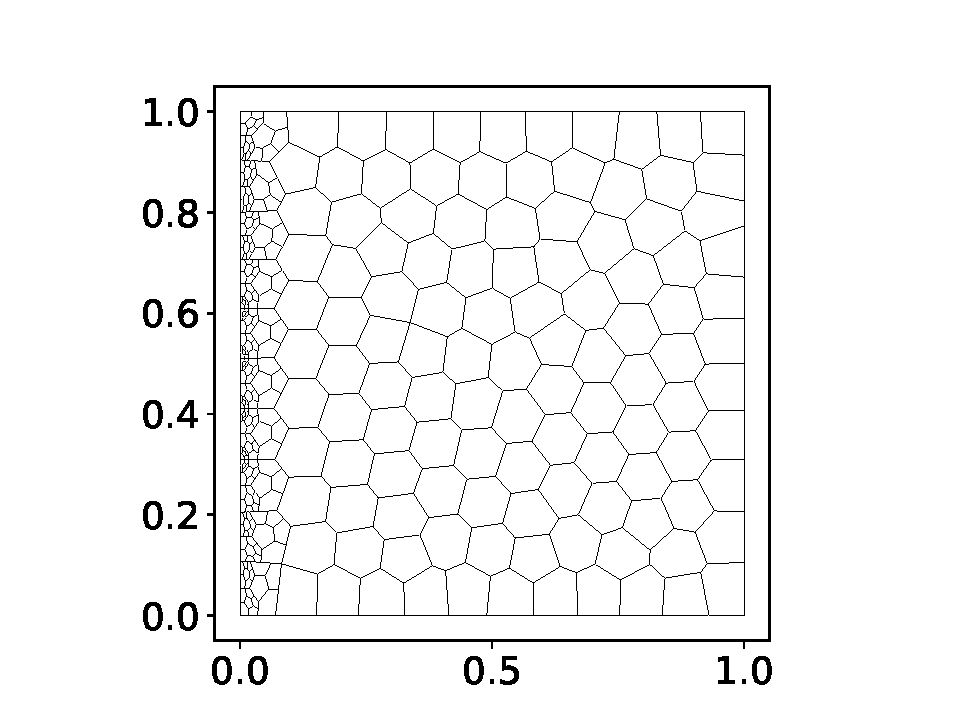
\includegraphics[width=5.5cm]{meshes/adaptive/square_eh_10.pdf}
	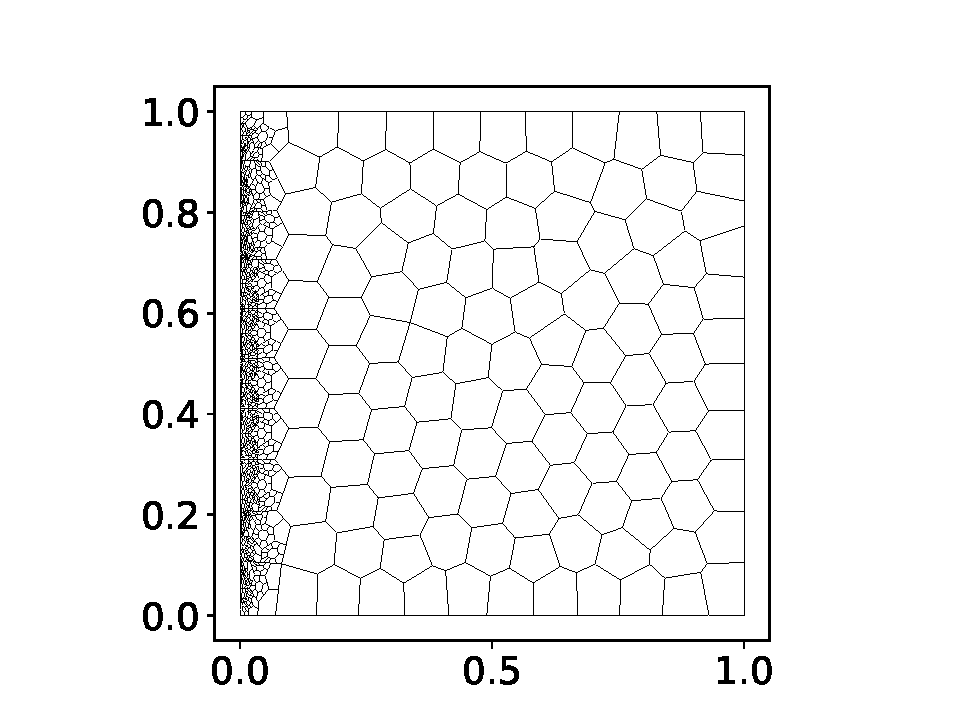
\includegraphics[width=5.5cm]{meshes/adaptive/square_eh_20.pdf}
	\caption{Square mesh after 5, 10 and 20 refinements, $N_0 = 125$.}
\end{figure}

\begin{figure}[!ht]
	\centering
	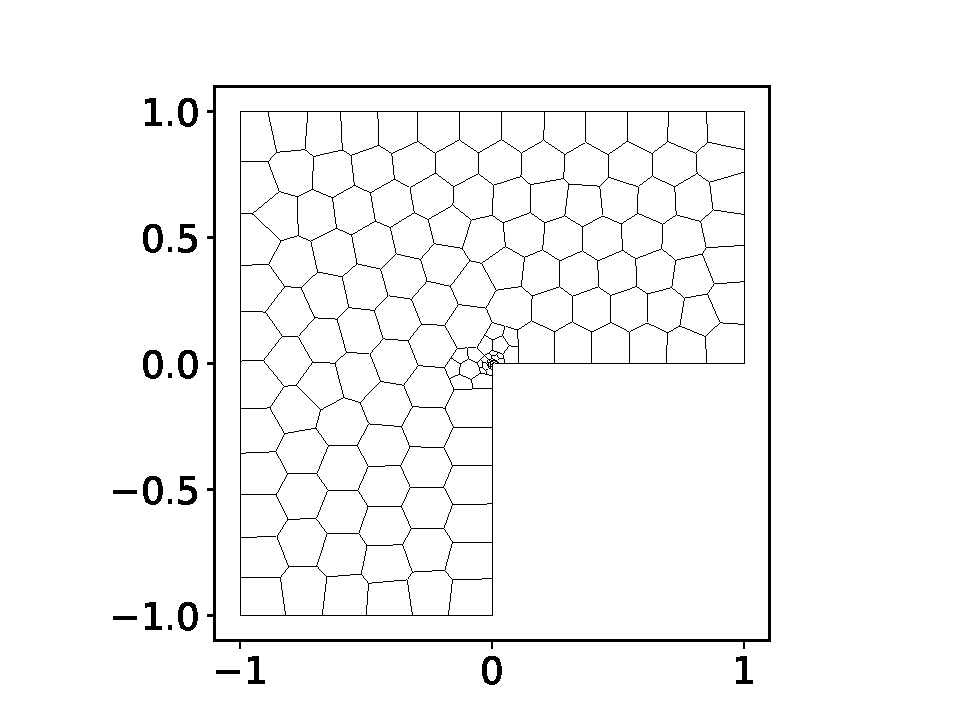
\includegraphics[width=5.5cm]{meshes/adaptive/lshape_eh_5.pdf}
	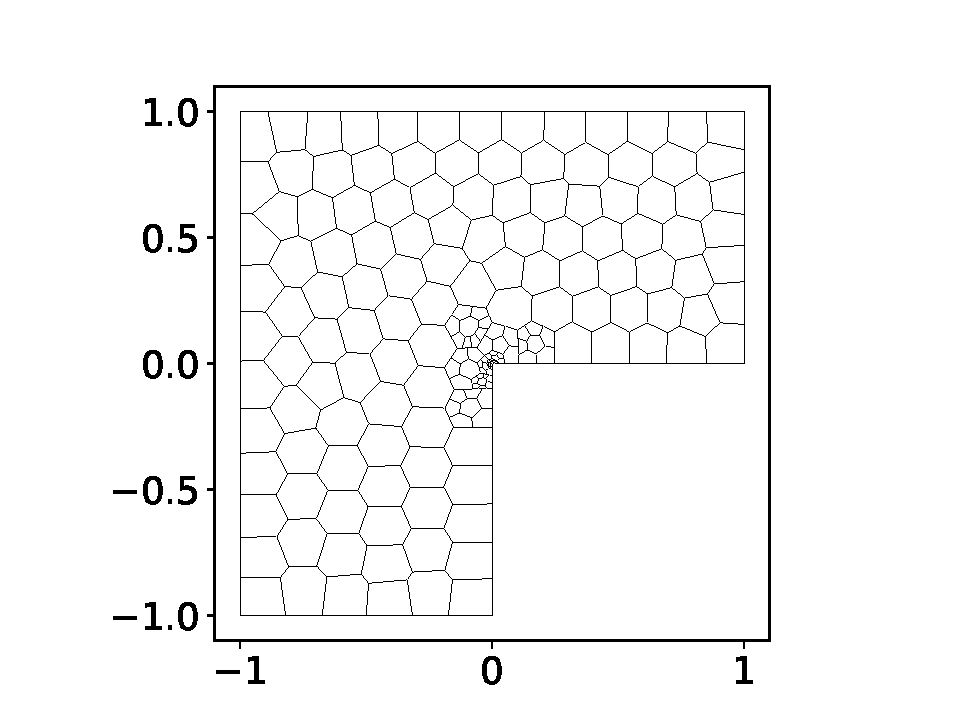
\includegraphics[width=5.5cm]{meshes/adaptive/lshape_eh_10.pdf}
	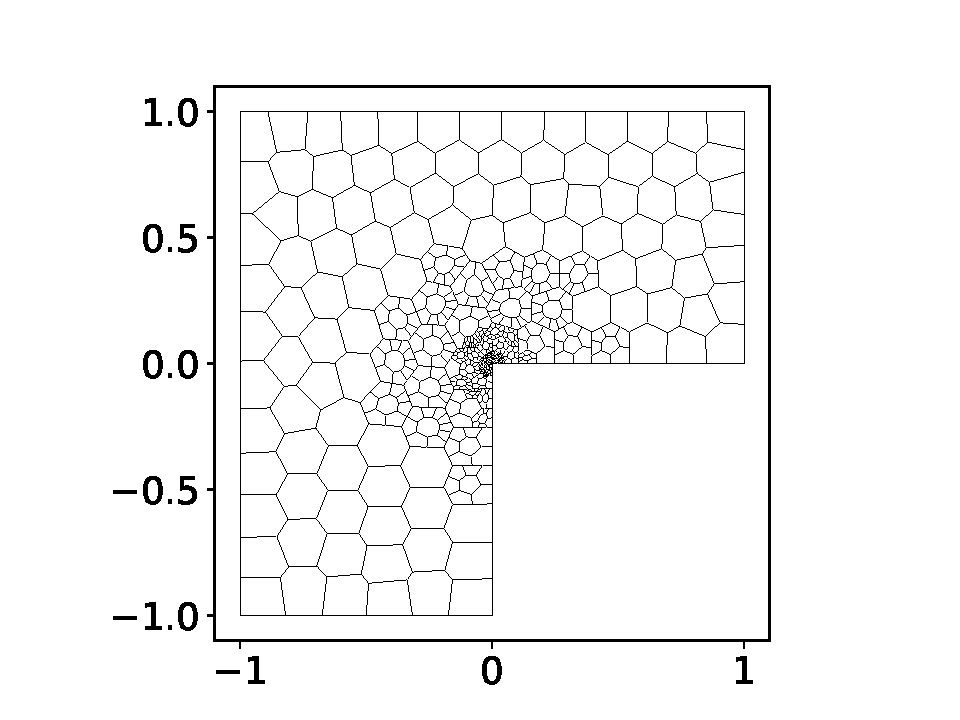
\includegraphics[width=5.5cm]{meshes/adaptive/lshape_eh_20.pdf}
	\caption{L-shaped mesh after 5, 10 and 20 refinements, $N_0 = 125$.}
\end{figure}

\newpage
\subsection{A code snippet}

Here's a snippet to illustrate the \textit{h-adaptive} mesh refinement from the user's perspective:

\lstinputlisting[style=cpp, firstline=11]{../snippets/h_refine.cpp}